\documentclass[border=4pt]{standalone}
\usepackage{tikz}
\usepackage{pgfplots}
\pgfplotsset{compat=1.17}
\usepackage[table]{xcolor}
\usetikzlibrary{shapes.geometric, arrows.meta, positioning, fit, calc}
\definecolor{headingblue}{HTML}{1F4E79}
\definecolor{lightblue}{HTML}{D9EAF7}
\definecolor{softgray}{HTML}{F4F6F8}
\definecolor{darkgray}{HTML}{404040}
\definecolor{prismagreen}{HTML}{E8F5E9}
\definecolor{prismabox}{HTML}{1565C0}
\definecolor{chartblue}{HTML}{2196F3}
\definecolor{chartorange}{HTML}{FF9800}
\definecolor{chartgreen}{HTML}{4CAF50}
\definecolor{chartred}{HTML}{F44336}
\definecolor{chartpurple}{HTML}{9C27B0}
\definecolor{chartgray}{HTML}{9E9E9E}
\begin{document}
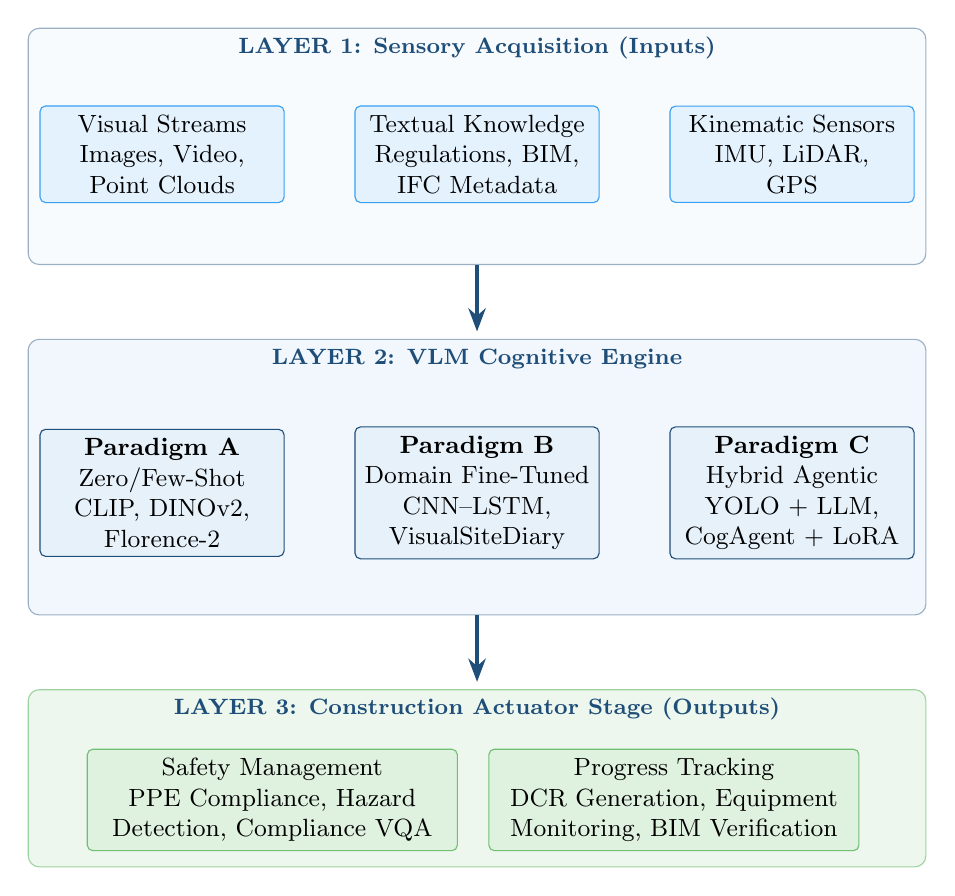
\begin{tikzpicture}[
  inp/.style={rectangle, draw=chartblue!90, fill=chartblue!12,
              rounded corners=2pt, minimum width=3.1cm, minimum height=1.1cm,
              align=center, font=\small},
  eng/.style={rectangle, draw=headingblue, fill=lightblue!65,
              rounded corners=2pt, minimum width=3.1cm, minimum height=1.6cm,
              align=center, font=\small},
  onode/.style={rectangle, draw=chartgreen!80, fill=chartgreen!18,
              rounded corners=2pt, minimum width=4.7cm, minimum height=1.2cm,
              align=center, font=\small},
  arr/.style={-Stealth, very thick, color=headingblue},
  hdr/.style={font=\footnotesize\bfseries\color{headingblue}},
]
%% --- Layer 1 background ---
\fill[lightblue!18, rounded corners=4pt] (-0.3, 1.0) rectangle (11.1, -2.0);
\draw[headingblue!45, rounded corners=4pt] (-0.3, 1.0) rectangle (11.1, -2.0);
\node[hdr] at (5.4, 0.75) {LAYER 1: Sensory Acquisition (Inputs)};

\node[inp] (i1) at (1.4, -0.6) {Visual Streams\\Images, Video,\\Point Clouds};
\node[inp] (i2) at (5.4, -0.6) {Textual Knowledge\\Regulations, BIM,\\IFC Metadata};
\node[inp] (i3) at (9.4, -0.6) {Kinematic Sensors\\IMU, LiDAR,\\GPS};

%% --- Arrow L1 → L2 ---
\draw[arr] (5.4,-2.0) -- (5.4,-2.85);

%% --- Layer 2 background ---
\fill[lightblue!38, rounded corners=4pt] (-0.3, -2.95) rectangle (11.1, -6.45);
\draw[headingblue!45, rounded corners=4pt] (-0.3, -2.95) rectangle (11.1, -6.45);
\node[hdr] at (5.4, -3.2) {LAYER 2: VLM Cognitive Engine};

\node[eng] (pa) at (1.4, -4.9) {\textbf{Paradigm A}\\Zero/Few-Shot\\CLIP, DINOv2,\\Florence-2};
\node[eng] (pb) at (5.4, -4.9) {\textbf{Paradigm B}\\Domain Fine-Tuned\\CNN--LSTM,\\VisualSiteDiary};
\node[eng] (pc) at (9.4, -4.9) {\textbf{Paradigm C}\\Hybrid Agentic\\YOLO + LLM,\\CogAgent + LoRA};

%% --- Arrow L2 → L3 ---
\draw[arr] (5.4,-6.45) -- (5.4,-7.3);

%% --- Layer 3 background ---
\fill[chartgreen!10, rounded corners=4pt] (-0.3, -7.4) rectangle (11.1, -9.65);
\draw[chartgreen!55, rounded corners=4pt] (-0.3, -7.4) rectangle (11.1, -9.65);
\node[hdr] at (5.4, -7.65) {LAYER 3: Construction Actuator Stage (Outputs)};

\node[onode] (o1) at (2.8, -8.8) {Safety Management\\PPE Compliance, Hazard\\Detection, Compliance VQA};
\node[onode] (o2) at (7.9, -8.8) {Progress Tracking\\DCR Generation, Equipment\\Monitoring, BIM Verification};
\end{tikzpicture}
\end{document}
